\documentclass[a4paper,notitlepage]{report}
\usepackage{url}
\usepackage{parskip}
\usepackage{graphicx}
\usepackage{float}
\usepackage{tikz}
\usepackage{circuitikz}
\usetikzlibrary{decorations.pathreplacing}
\usetikzlibrary{patterns}
\usepackage{listings}
\usepackage{color}
\definecolor{lightgray}{rgb}{.9,.9,.9}
\definecolor{darkgray}{rgb}{.4,.4,.4}
\definecolor{purple}{rgb}{0.65, 0.12, 0.82}
\lstdefinelanguage{JavaScript}{
  keywords={break, case, catch, continue, debugger, default, delete, do, else, false, finally, for, function, if, in, instanceof, new, null, return, switch, this, throw, true, try, typeof, var, void, while, with},
  morecomment=[l]{//},
  morecomment=[s]{/*}{*/},
  morestring=[b]',
  morestring=[b]",
  ndkeywords={class, export, boolean, throw, implements, import, this},
  keywordstyle=\color{blue}\bfseries,
  ndkeywordstyle=\color{darkgray}\bfseries,
  identifierstyle=\color{black},
  commentstyle=\color{purple}\ttfamily,
  stringstyle=\color{red}\ttfamily,
  sensitive=true
}

\lstset{
   language=JavaScript,
   backgroundcolor=\color{lightgray},
   extendedchars=true,
   basicstyle=\footnotesize\ttfamily,
   showstringspaces=false,
   showspaces=false,
   numbers=left,
   numberstyle=\footnotesize,
   numbersep=9pt,
   tabsize=2,
   breaklines=true,
   showtabs=false,
   captionpos=b
}

\begin{document}

\title{Logic Circuit Workbench: GatePlay}
\author{Greg O'Connor \\
		Computer Science, University of Oxford \\
		\\
		Third Year Project\\
		Supervisor: Geraint Jones}
\date{\today}
\maketitle

\begin{abstract}
GatePlay is an application to build and simulate logic circuits from within the web browser, without the need for installation or extra plug-ins. It is designed to couple a simple and aesthetically pleasing Graphical User Interface with an efficient and accurate simulation.
\end{abstract}
\clearpage

\tableofcontents
\clearpage

\chapter{Introduction}

\section{Motivation}
Logic circuits underpin practically every aspect of modern life in the form of computer chips. It is therefore important that people have the opportunity to learn about and understand logic circuits.

I believe that one of the best ways to learn about logic circuits is to build them, and that the most accessible way of doing that is by using a simulated workbench --- avoiding the cost and expertise required to build physical circuits. The workbench is not designed to be used by professionals in designing chips, but for casual users looking to learn about logic circuitry.

Projects which attempt to solve the same problem can already be found on the Internet. Two of the best examples I could find were Logic.ly\footnote{http://logic.ly} and CircuitLab\footnote{http://www.circuitlab.com}.

Logic.ly was easy to use but had two major problems. First and foremost, the simulation implemented in Logic.ly over simplified: it does not assign any propagation delay to its components, making it difficult to see what happens in oscillating circuits. Secondly, it is implemented using Adobe Flash. Flash requires a web browser plug-in not included on many devices (notably iOS devices), which reduces Logic.ly's accessibility.

CircuitLab is more at more power users and has a much steeper learning curve than Logic.ly. CircuitLab also allows users to create general electronic circuits from power sources, resistors, etc. which adds to the complexity of the user interface.

Therefore I decided to build a workbench which is easy to use but would not simplify the simulation more than necessary.

\section{Overview of GatePlay}
GatePlay can be seen in figure~\ref{fig:interface}. The labelled regions are:

\begin{itemize}
	\item[1] The \textbf{top bar}, which has buttons to download the workbench as an image and to start simulating the circuit. When simulating, the top bar has additional controls such as starting, restarting, and pausing the simulation.
	\item[2] The \textbf{left bar}, which has sliding panels containing the  components available to build circuits with. The user simply drags a gate from the left bar onto the workbench to add it to the circuit.
	\item[3] The \textbf{workbench}, which is where almost all interaction with GatePlay happens. When editing you can move, delete, and draw wires between components. When simulating the values of wires are shown visually on the workbench.
\end{itemize}

The components and wires on the workbench snap to the grid lines which can be seen in the screenshots.

GatePlay has a library of standard components which can be used to build circuits. All of the components are implemented as black boxes, even though most of them can be re-implemented using a combination of the simpler components.

\begin{itemize}
	\item \textbf{Input} components such as constant $ON$, $Toggle$ (clicking on a $Toggle$ during simulation will change its value), and $Blinker$ (which flip their value at a constant interval)
	\item \textbf{Output} components such as $LED$s. Outputs allow the workbench to capture the intended output of a circuit, and display it to the user.
	\item \textbf{Gates} implement standard boolean logic functions such as $NOT$, $AND$, and $XOR$
	\item \textbf{Function} components such half adders and full adders
	\item \textbf{Memory} components such as SR latches and D flip-flop  
\end{itemize}

A typical workflow for creating circuits would be:

\begin{enumerate}
	\item Drag the desired components from the left-bar on to the workbench
	\item Wire the components up by left-clicking on output ports, and then left-clicking on an input port. Fixed points can be created along the way by left-clicking on an empty part of the workbench
	\item Entering simulation mode by clicking on the "Start Simulating" button on the top-bar
	\item The simulation can now be paused, resumed, or advanced manually by using the controls in the top-bar
	\item The user may decide to return to editing mode to add, move, or delete components, or re-wire parts of the circuit.
\end{enumerate}

Figure~\ref{fig:dflopflop} shows a D flip-flop being simulated on the workbench. Green wires are $High$ (logical $True$) and red wires are $Low$ (logical $False$). The round components on the left are $Toggle$s; clicking them will change their value and cause the resulting changes to propagate through the circuit.

\begin{figure}[p]
    \centering
    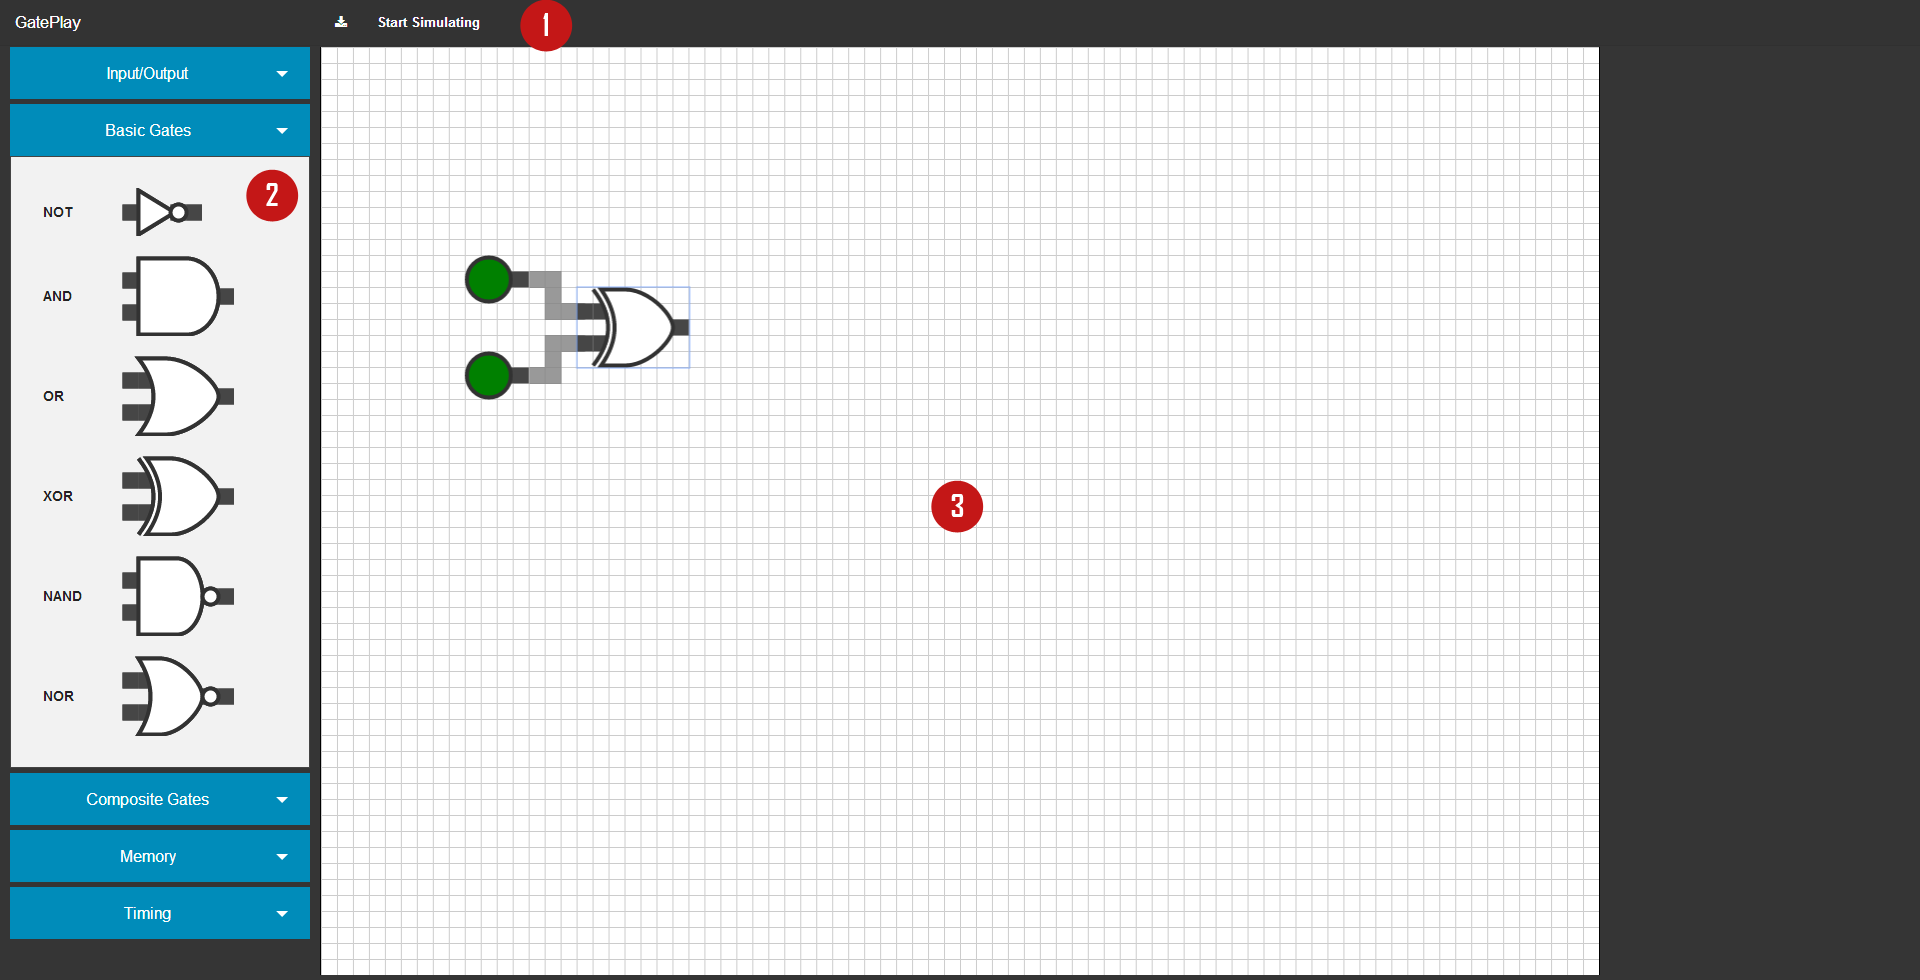
\includegraphics[width=\textheight,angle=270]{labelled.png}
    \caption{Drawing a circuit}
    \label{fig:interface}
\end{figure}

\begin{figure}[p]
    \centering
    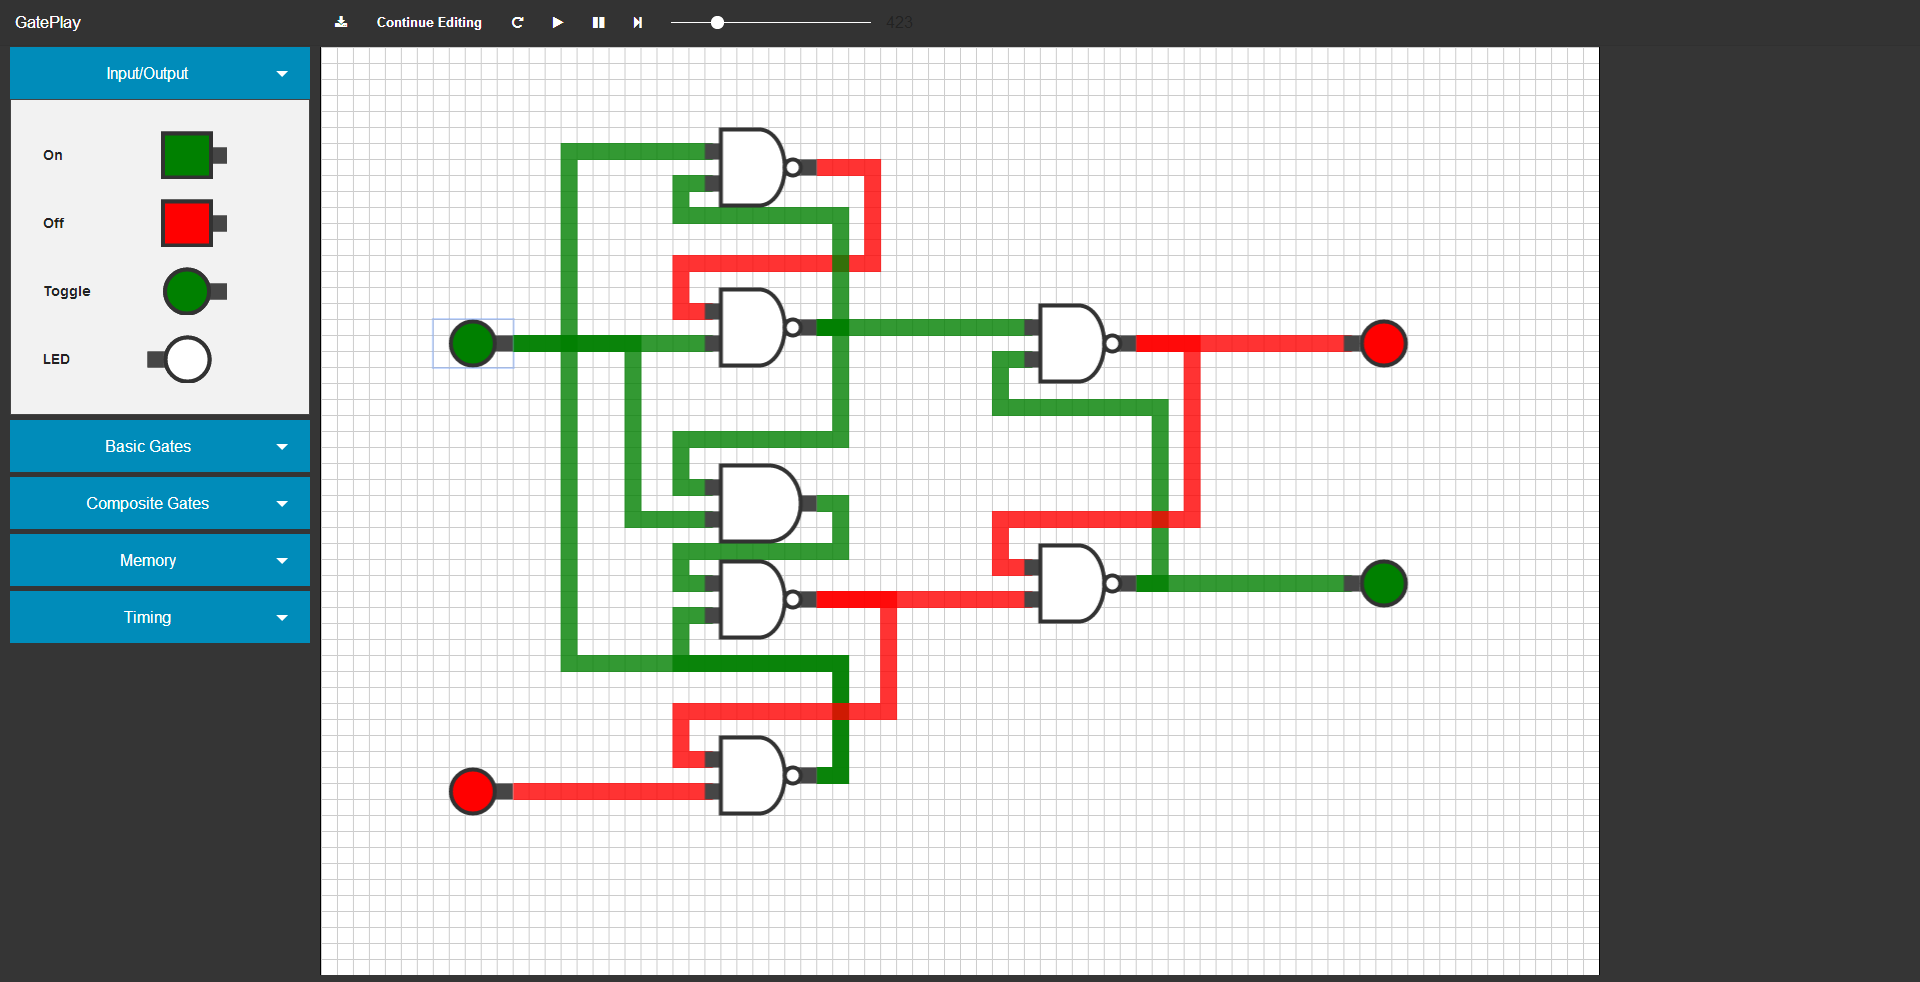
\includegraphics[width=\textheight,angle=270]{dflipflop.png}
    \caption{Simulating a D flip-flop}
    \label{fig:dflopflop}
\end{figure}
\clearpage
\chapter{Background}
\label{chapter:background}

\section{Logic Circuits}
\label{sec:circuits}
A \textit{k-ary Boolean function} is a function which take $k$ boolean values and returns a boolean value.
\[ F : \{True, False\}^k \rightarrow \{True, False\} \]
\textit{Logic gates} are physical implementations of (typically simple) boolean functions. A \textit{logic circuit} is a collection of logic gates wired together, producing an implementation of the composition of boolean functions.

By composing ever more complex functions we can create physical implementations of useful circuits --- for example circuits which add or multiply the binary representation of numbers.

A logic gate has a \textit{propagation delay} defined as the time from when its inputs become stable and valid to when its outputs become stable and valid. Propagation delay changes based on temperature, voltage, and output capacitance (\cite{Wikipedia: Propagation Delay}).

\section{Building Websites}
GatePlay is a web application. Instead of being installed on the user's computer it runs in their web browser. GatePlay is a single HTML document and has relatively few CSS style rules. The vast majority of the work was creating the JavaScript, which handles all interactions with the top and left bars, as well as displaying, editing, and simulating circuits.

\begin{itemize}
	\item[HTML] defines the semantic structure of the website as a collection of nested elements, known as the DOM (Document Object Model) tree. In other words, HTML defines the content of a website and the structure of headings, sections, paragraphs, etc.
	
	\item[CSS] Cascading Style Sheets modify how HTML documents are displayed by the clients browser. CSS files are lists of \textit{selectors} with associated \textit{attributes}. A selector describes elements based on their position in the DOM tree, and its attributes modify how those elements are displayed. For example, it is easy to specify the following styles in CSS: ``All elements of type \textit{gate} should be 150 pixels wide'', or ``The middle section of the website should take up 80 percent of the width''.
	
	\item[JavaScript] JavaScript is a full programming language which is run in the user's browser when they load the website. It can perform arbitrary computations, and is also free to modify the structure of the  DOM tree and the styles of elements.
\end{itemize}

\subsection{JavaScript}
JavaScript is as dynamic, imperative programming language which can run in all modern web browsers. The code listings included in this report should be understandable to those familiar with languages such as C++ or Java.

JavaScript is an example of Prototype-based programming\footnote{http://en.wikipedia.org/wiki/Prototype-based\_programming}. In the code listings of this report, lines such as ``MyClass.prototype.myMethod = function(...) { ... }'' can be thought of simply as adding the method \textit{myMethod} to the class definition of \textit{MyClass}.
\clearpage
\chapter{Requirements}
It was agreed that the project should satisfy the following requirements:

\begin{itemize}
	\item[Accessible]
	\begin{itemize}
		\item[Web Based]
		\item[Plugin Free]
		\item[Simple UI]
	\end{itemize}
	
	\item[Non-simplistic simulation]
\end{itemize}


\clearpage
\chapter{Simulation}
\label{chapter:simulation}

\section{Modelling Circuits}
A circuit can be modelled as a set of components and a set of wires. The fields which define components and wires are shown in figures \ref{fig:component} and \ref{fig:wire} respectively. The only constraint placed on circuits is that no more than one wire may go into the same input port.

\begin{figure}[H]
\centering
\begin{itemize}
	\item The \textbf{number of inputs} the component has ($N$)
	\item The \textbf{number of outputs} the component has ($M$)
	\item An \textbf{evaluation function} which takes a list of $N$ truth values and returns a list  of $M$ truth values. The Evaluation Function also defines the propagation delay of the component, as discussed throughout this chapter.
\end{itemize}
\caption{Fields of a Component}
\label{fig:component}
\end{figure}

\begin{figure}[H]
\centering
\begin{itemize}
	\item The \textbf{source component} the wire is leaving from
	\item The \textbf{output port} of the source component
	\item The \textbf{target component} the wire is going to
	\item The \textbf{input port} of the target component
	\item The current \textbf{truth value} of the wire 
\end{itemize}
\caption{Fields of a Wire}
\label{fig:wire}
\end{figure}

\section{Event-Based Simulation}
GatePlay uses an event-based algorithm to simulate logic circuits. An event is a notification that a specific output of a component has changed. They are defined by the following four values:

\begin{itemize}
	\item The \textbf{source component} the event is propagating from
	\item The \textbf{output port} on the source component which has changed value
	\item The \textbf{event time} at which it is occurring
	\item The new \textbf{truth value} of the output port
\end{itemize}

Events are stored in a priority queue, and have priority equal to their event time. Lower times are more urgent. 

\subsection{Initial Components}
\label{subsec:initial}
The first events in a simulation run are generated by so called \textit{Initial Components}. An initial component is defined as a component which takes no inputs. Some examples of initial components are described below:

\begin{itemize}
	\item \textbf{Constant Components} such as $ON$ and $OFF$ never change value, and so place their events in the queue just once when the circuit is initialised.
	
	\item \textbf{Timed Components} such as $Blinker$s toggle their output at a set interval. The algorithm to do so is non-trivial and discussed in chapter~\ref{chapter:implementation}.
	
	\item \textbf{External Components} like $Toggle$s add events based on user interaction. Since the stimulus to create an event comes from outside the simulator, it is a simple case of putting a method to create circuit events in the circuit's public API.
\end{itemize}

The heart of an event-based simulation is the event loop which processes all the events and generates new events.

\begin{figure}[H]
\begin{enumerate}
	\item \textbf{Fetch} next event to be processed from priority queue
	\item \textbf{Update} the value of the wires connected to the event port
	\item \textbf{Recalculate} the output of any gates whose inputs changed
	\item \textbf{Propagate} the change by creating new events for each changed output, and add to the queue after the gate's delay
\end{enumerate}
\caption{Event Loop Body}
\end{figure}

\subsection{Event Loop Example}
Consider the circuit shown in figure~\ref{fig:simple}. Let $X$'s current output be $False$, the event queue contain a single event $ev = (X, 1, t, True)$, and the current time be $t$.

\begin{figure}[H]
\centering
\begin{circuitikz} \draw
	(1,0) node[not port] (not1) {}
	(3,0) node[not port] (not2) {}
	(not1.out) -- (not2.in);
	\draw (not1) node[left=-2pt] {X};
	\draw (not2) node[left=-2pt] {Y};
\end{circuitikz}
\caption{Two $NOT$ Gates}
\label{fig:simple}
\end{figure}

When the event look body executes, the following actions occur:

\begin{enumerate}
	\item Pop $ev$ from the queue
	\item Update the wire coming from $X$ port $1$ to $True$
	\item $A$ enters $Y$, so its input has changed. Apply $Y$'s evaluation function to the new input, which returns $False$
	\item Since $Y$'s output changed, add the following new event to the queue: $(Y, 1, t + \delta, False)$ where $\delta$ is $Y$'s gate delay
\end{enumerate}

As the event loop repeats, changes propagate through a circuit.

\subsection{Culling}
\label{subsec:culling}
Events can sometimes be discarded without being processed by the entire event loop. For example, events which set an output port to the value it already is do not change anything in the circuit and can be discarded during stage 2 of the event loop.

\subsection{Event Race Conditions}
Consider the circuit shown in figure~\ref{fig:racecondition}:
\begin{figure}[H]
\centering
\begin{circuitikz} \draw
	(1,0) node[and port] (and1) {}
	(and1.in 1) node[anchor=east]{False - A}
	(and1.in 2) node[anchor=east]{False - B}
	(and1.out) node[anchor=west]{C - False};
	 \draw (and1) node[left=12pt] {Z};
\end{circuitikz}
\caption{AND gate}
\label{fig:racecondition}
\end{figure}

Suppose there are two events in the event queue: $ev_1 = (X, 1, t, True)$ and $ev_2 = (Y, 1, t, True)$ where $X$ port $1$ is wired to $A$, and $Y$ port $1$ is wired to $B$.  In other words, A and B both become $True$ at time $t$. Now consider what happens in the event loop at time $t$.

We handle each event independently, so suppose we handle $ev_1$ first: We set $A$ to $True$, $B$ is still thought to be $False$, and therefore we add the event $(Z, 1, t + \delta, False)$ to the queue (as $True \land False = False$).

Next we handle $ev_2$: $B$ is set to $True$ and $A$ is known to be $True$, so we add the event $(Z, 1, t + \delta, True)$ to the queue (as $True \land True = True$).

The queue now contains two events with different truth values occurring on $Z$ port $1$ at the same time. If the event valued at $False$ is handled first it will be culled and the circuit will be simulated correctly. However if it is handled second then the output of $Z$ will be calculated as $False$, despite both its inputs being $True$! Since we are using a priority queue and both events have the same priority, there is no defined behaviour for which event will be handled first.

The solution is to do a first pass through all events happening at time $t$ and update the values of each of the affected wires. Now if we process $ev_1$: $A$ and $B$ are already set to $True$ because of the first pass, and we calculate $Z$'s output to be $True$. Handling $ev_2$ will again yield $True$, and one of the duplicate events will be culled.

There is a further refinement implemented in GatePlay: when we do the initial pass through all events happening at time $t$ we maintain a set --- sets do not store duplicate values --- of all affected components. In this example both events only affect $Z$, so the set will be $\{Z\}$. We then re-calculate the output of each component in the set and add the event to the queue. In this case, we will only calculate and add $(Z, 1, t + \delta, True)$ once.

\subsection{Efficiency}
The speed of an event-based simulation is proportional to the number of events being generated and processed. For this reason, reducing the time spend processing events through Culling (see section~\ref{subsec:culling}) is critically important.

Also note that (if sensible data structures are used) event-based simulations are still performant in circuits with very large number of components and connections, so long as relatively few events are occurring. An efficient simulation is not necessary for GatePlay as the UI only allows users to build modest-sized circuits, but it is good to implement an efficient simulator regardless in case the UI is ever changed.

\section{2-Valued Simulation}
\label{sec:2-valued}
\subsection{Description}
A simple simulation of logic circuits might use a 2-valued simulation. Each wire has one of two values: \textit{True} or \textit{False}. While it provides a reasonable model for logic circuits, it has some limitations described in this section.

\subsection{Initialisation Values}
\label{subsec:2-valued initialisation}
In a 2-valued simulation all wires must be either $True$ or $False$ valued. It is necessary to initialise the wire values before the circuit begins, but what is a sensible default? Suppose we initialise all wires to $False$, and consider the circuit in figure~\ref{fig:initialisation}:

\begin{figure}[H]
\centering
\begin{circuitikz} \draw
	(1,0) node[not port] (not1) {}
	(not1.in) node[anchor=east] {False}
 	(not1.out) node[anchor=west] {False};
\end{circuitikz}
\caption{An inconsistently initialised $NOT$ Gate}
\label{fig:initialisation}
\end{figure}

To have both $A$ and $B$ both be initialised to be $False$ is inconsistent with the logic of the circuit. The same would be true is wires were initialised to $True$. One option would be to add a boolean flag to wires indicating that no event has reach them yet, and leave them uninitialised at first, however there is a more suitable solution introduced in section~\ref{sec:3-valued}.


\subsection{Propagation Delay Uncertainty}
\label{subsec:2-valued uncertainty}
As discussed in section~\ref{sec:circuits}, the \textit{Propagation Delay} of a component is the time it takes from its inputs being stable and valid to its outputs becoming stable and valid (from Wikipedia). 

Previously we have assumed that this delay is constant for a given component, but in reality the precise delay varies based on temperature, voltage, and output capacitance. Our model of logic circuits does not consider these factors and therefore cannot make an informed estimation of the delay for each pass through a component.

For example, suppose the $NOT$ gate shown figure~\ref{fig:2-valued-circuit} never has a propagation delay of less than $\delta_{min}$ nor a delay of greater than $\delta_{max}$.

\begin{figure}[H]
\centering
\begin{circuitikz} \draw
	(1,0) node[not port] (not1) {}
	(not1.in) node[anchor=east] {A}
 	(not1.out) node[anchor=west] {B};
\end{circuitikz}
\caption{A $NOT$ Gate}
\label{fig:2-valued-circuit}
\end{figure}

\begin{figure}[H]
\centering
	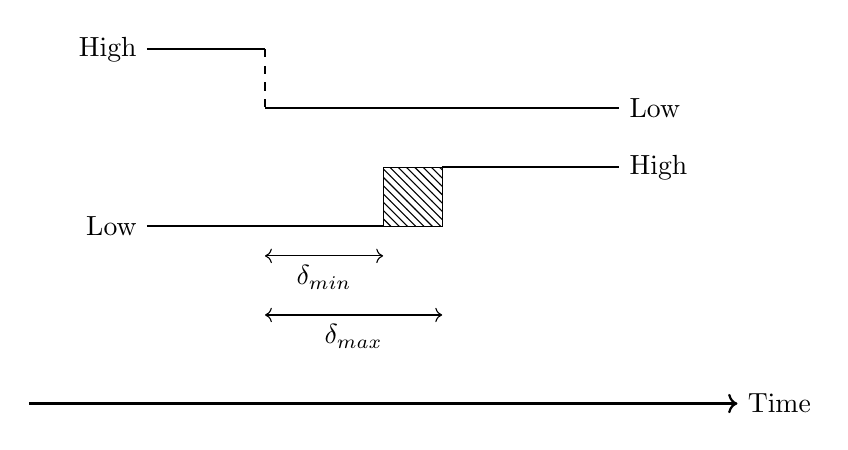
\begin{tikzpicture}[domain=0:4, xscale=1.5, yscale=0.75] 
   		\draw [thick] (0,1) node[left] {High} -- (1,1);
    	\draw [thick, dashed] (1,1) -- (1,0);
    	\draw [thick] (1,0) -- (4,0) node[right] {Low};
    	\draw [thick] (0,-2) node[left] {Low} -- (2,-2);
    	\draw [pattern=north west lines] (2,-2) rectangle (2.5,-1);
    	\draw [thick] (2.5,-1) -- (4,-1) node[right] {High};
    	\draw [thick,->] (-1,-5) -- (5,-5) node[right] {Time}; 
    	\draw [<->] (1,-2.5) -- (2,-2.5) 
			node [pos=0.5,anchor=north] {$\delta_{min}$};
		\draw [<->]	(1,-3.5) -- (2.5,-3.5) 
			node [pos=0.5,anchor=north] {$\delta_{max}$};
	\end{tikzpicture}
	\caption{2-valued Low-High transition}
	\label{fig:2-valued-trace}
\end{figure}

If we flip A's value from $True$ top $False$ the trace of the truth values through time is shown in figure~\ref{fig:2-valued-trace}. $B$'s transition from Low to High can happen at any point in hatched region based on the aforementioned factors. A 2-valued simulator at this level of detail can therefore only assume that the transition happens at a random time. In other words, the precise propagation delay for each pass through a component is randomly sampled from interval $[\delta_{min}, \delta_{max}]$.

Each simulation of a circuit will likely have different propagation delays which can potentially change the output of a circuit altogether. If a run of this one simulation yields a given result there is no guarantee that \textit{all} runs would yield the same result. I felt this was not desirable behaviour for a simulator. In the next section we introduce a simulator which models the uncertainly of components without introducing non-determinism in the simulation itself.

\section{3-Valued Simulation}
\label{sec:3-valued}
The way I decided to overcome the problems of 2-valued simulation (see section~\ref{sec:2-valued}) was to instead use a 3-valued simulation. A wire has one of three values: $True$, $False$, $Unknown$. A wire that is $Unknown$ may "in reality" be either true or false, but the simulation does not know which.

\subsection{Initialisation Values}
In a 3-valued simulation all wires can be initialised to $Unknown$ without the problem of inconsistency for 2-valued simulations discussed in section~\ref{subsec:2-valued initialisation}.

\subsection{Propagation Delay Uncertainty}
\label{subsec:3-valued uncertainty}
The 2-valued simulation was unable to model the uncertainty of component delay without making the result of each simulation run non-deterministic as discussed in section~\ref{subsec:2-valued uncertainty}.

Suppose we have a component $X$ whose inputs are changing at time $t$. In the 2-valued simulation we would consider the outputs changing at time $t + \delta$ where $\delta$ is randomly sampled from the interval $[\delta_{min}, \delta_{max}]$. 

However in the 3-valued simulation we can consider the outputs of $X$ to be changing twice. At time $\delta_{min}$ they becoming $Unknown$, and then at time $\delta_{max}$ they settle on a stable value. 

By considering the output $Unknown$ for the duration of the delay uncertainty we have still modelled the uncertainty in the actual components, but without introducing uncertainty to our simulation. In other words, should a circuit yield a certain value in our simulation we know that it will yield a certain value for \textit{all} possible combinations of gate delays.

\subsection{Event Suppression}
A bug was introduced in the simulator in section~\ref{subsec:3-valued uncertainty}. Consider the circuit shown in figure~\ref{fig:suppression}. Let $\delta_{min}$ and $\delta_{max}$ be the minimum and maximum gate delay respectively. $A$, $B$, and $C$ are all $False$.

\begin{figure}[H]
\centering
\begin{circuitikz} \draw
	(1,0) node[and port] (and1) {}
	(and1.in 1) node[anchor=east] {A}
	(and1.in 2) node[anchor=east] {B}
 	(and1.out) node[anchor=west] {C};
\end{circuitikz}
\caption{An $AND$ Gate}
\label{fig:suppression}
\end{figure}

Let circuit event $e_1$ set $A$ to $True$ at time $t$, and event $e_2$ set $B$ to $True$ at time $t + 1$. Using the algorithm thus far described we will handle $e_1$ and the following two events will be added to the queue: $e_3 = (X, 1, t + \delta_{min}, Unknown)$, $e_4 = (X, 1, t + \delta_{max}, False)$. Next, handling $e2$ we will add these events to the queue: $e_5 = (X, 1, t + 1 + \delta_{min}, Unknown)$, $e_6 = (X, 1, t + 1 + \delta_{max}, True)$.

The bug arises at time $t + \delta_{max}$ when we handle $e_4$. At that time $C$ is set to $Unknown$ and we will set it to $False$. However this is incorrect behaviour as $e_2$ means that $C$ should be uncertain until $e_6$ is handled at time $t + 1 + \delta_{max}$.

In other words, the output of X is uncertain for two distinct reasons. $e_1$ causes $C$ to be uncertain in the interval $[t + \delta_{min}, t + \delta_{max})$, and $e_2$ makes it uncertain in the interval $[t + 1 +  \delta_{min}, t + 1 + \delta_{max})$.

The simulator therefore must keep track of the intervals a wire is uncertain for, and \textit{suppress} any events which try to set it to a certain value in any of those intervals. In this example $e_4$ must be suppressed.
\clearpage
\chapter{Implementation}
\label{chapter:implementation}
Make some general points here

\section{Getting Started}

\subsection{Require.js}
When the GatePlay url is visited, the only file downloaded is the main HTML file: index.html. The index then directs the user's browser to download the additional CSS and JavaScript files needed to use GatePlay.

A JavaScript script may use methods or variables defined in the global namespace, even if they were put there by another script, provided that the script has already been run.

\begin{figure}[H]
\begin{lstlisting}[language=html]
<!-- componentview depends on component -->
<!-- Therefore we ensure component is loaded first -->
<script type="text/javascript" src=".../component.js"></script>
<script type="text/javascript" src=".../componentview.js"></script>
\end{lstlisting}
\caption{Example use of Script tags}
\end{figure}

It is time consuming for a human to find and type out a correct ordering for the Script tags, and it would need to be updated every time a file as added or removed, or sometimes if a file were modified.

Require.js is a JavaScript file loader which does automatically loads files in a correct order. Each JavaScript file declares each of its direct dependencies, and Require.js will ensure they are all loaded correctly when the webpage loads.

\begin{figure}[H]
\begin{lstlisting}[language=JavaScript]
// componentview.js

require([
	// Declare the path of each file we require	
	"canvas/model/component"
], function(Component) {
	// Each included file is run, and we can give a name to whatever it returns if desired
	var myComponent = new Component();
	...
});
\end{lstlisting}
\caption{An example file which uses Require.js}
\end{figure}

\section{The Workbench}

GatePlay's workbench is where we create and view circuits, and is implemented using an HTML Canvas element. A canvas is a blank slate which can have shapes and images drawn using the JavaScript API.


\subsection{Fabric.js}
An HTML Canvas only provides low level drawing tools. You are able to draw shapes and images on it, but there is no concept of persist objects on the canvas.

Fabric.js is a library which wraps HTML Canvases with an object model, allowing GatePlay to interact at the level of objects being added to, modified, and remove from the canvas, rather thana  flat array of pixels.

Suppose I wanted to add a rectangle to a canvas, and then move it to a new location. Using Fabric.js this is two library calls (one to add a rectangle object and one to change the position property of the object). Using an HTML Canvas it is still one call to draw the rectangle, but moving it would require calculating what would be behind the rectangle, drawing that over the rectangle, and then re-drawing the rectangle at its new location. Fabric.js greatly reduces the amount of boilerplate code otherwise needed to interact with canvases.

Initially GatePlay used a different canvas framework called KineticJS, but due to difficulties getting features like snap-to-grid working I switched to Fabric.js.

\subsection{MVC with Backbone.js}
Model-view-controller\footnote{http://en.wikipedia.org/wiki/Model-view-controller} is a design pattern to simply program development. GatePlay uses MVC in the implementation of the workbench. MVC applications contain three types of components:

\begin{itemize}
	\item \textbf{Models} which store some part of the state of the application
	\item \textbf{Views} which display a representation of one of the models to the user
	\item \textbf{Controllers} which process user input, and updates the appropriate models.
\end{itemize}

The interactions between the components can be seen in figure~\ref{fig:mvc}. By separating out the concerns of the program it becomes possible to, for example, add new views for your models without needing to change the models or controllers themselves.

\begin{figure}[H]
	\centering
	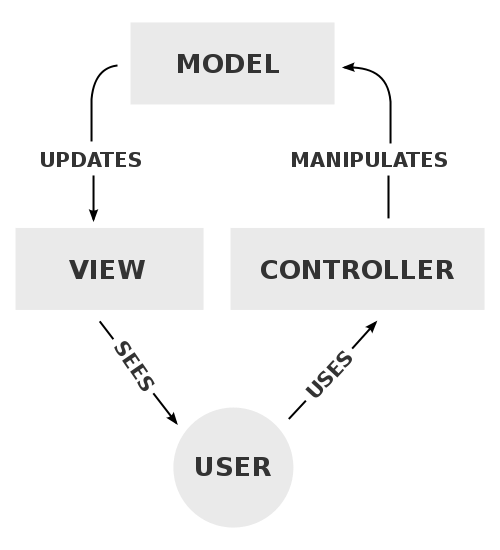
\includegraphics[width=0.5\textwidth]{mvc.png}
	\caption{Interaction of MVC Components, from Wikipedia}
	\label{fig:mvc}
\end{figure}

Backbone.js\footnote{http://backbonejs.org} is a JavaScript library to reduce the amount of boilerplate code in developing MVC JavaScript applications.

One model is the Wire model as shown in figure~\ref{fig:wiremodel}. It includes a lot of the same information as the Wire objects used in the simulation, but also includes information regarding the \textit{fixed points} of the wire.

We then create a view associated with the Wire model (figure~\ref{fig:wireview}). 

\begin{figure}
\begin{lstlisting}[language=JavaScript]
Backbone.Model.extend({
	defaults: function() {
    	return {
        	id: nextWireId++,
        	sourceId: -1,
        	sourcePort: -1,
       	 	targetId: -1,
        	targetPort: -1,
        	fixedPoints: [],
        	truthValue: TruthValue.UNKNOWN
    	}
	},
})
\end{lstlisting}
caption{Definition of a Wire model}
\label{fig:wiremodel}
\end{figure}

\begin{figure}
\begin{lstlisting}[language=JavaScript]
Backbone.View.extend({
    initialize: function(options) {
        // When the model is changed, update the view
        this.model.on("change:fixedPoints", this.render, this);
        this.model.on("change:truthValue", this._setWireColor, this);
    },

    render : function() {
        var model = this.model;
		
		// Using the model data we can now draw wires on the canvas
    },

    _setWireColor: function() {
        var truthValue = this.model.get("truthValue");
        
        // We can now re-render the wire with the new colour
    }
});
\end{lstlisting}
caption{Definition of a Wire view}
\label{fig:wireview}
\end{figure}


\subsection{Editing Mode}


\subsection{Running Mode}

\section{The Simulator}
The implementation of GatePlay's simulator is a relatively straightforward implementation of the algorithms and ideas explained in section~\ref{chapter:simulation}. The following six classes fully implement the simulator:

\begin{itemize}
	\item \textbf{truthvalue.js} defines constants $True$, $False$, and $Unknown$
	\item \textbf{component.js} defines a Component by its input count, output count, and evaluation function
	\item \textbf{wire.js} defines a Wire by its input component and port, output component and port, and truth value
	\item \textbf{circuitevent.js} defines a CircuitEvent by component, port, timestamp, and value
	\item \textbf{functions.js} contains definitions of all the Evaluation Functions available to the simulator 
	\item \textbf{circuit.js} is the only class which need be visible from outside the simulator. It has an interface to add components and wires. Circuit.js implements the algorithm for the event loop. 
\end{itemize}

\subsection{Blinker Events}
Recall section~\ref{subsec:initial} that $Blinker$ components toggle their output value at a set interval. Each $Blinker$ has its own, potentially unique, interval.

To implement this, a $Blinker$ component's evaluation function (shown in figure~\ref{fig:blinkereval} determines it truth value backed on the simulation clock.

\begin{figure}
\begin{lstlisting}[language=JavaScript]
Blinker.prototype._doEvaluate = function(argList, clock) {
    var period = Math.floor(clock / this._interval);
    var parity = period % 2;
    if (parity === 0) {
        return [TruthValue.TRUE];
    } else {
        return [TruthValue.FALSE];
    }
};
\end{lstlisting}
\caption{Implementation of $Blinker$'s evaluation function}
\label{fig:blinkereval}
\end{figure}

However a $Blinker$ will never be processed by the event loop, as no events will ever affect a $Blinker$ (it has no inputs). Therefore we need to handle $Blinker$s differently.

The solution implemented in GatePlay is to add a new circuit event for every $Blinker$, \textit{every} clock tick. For a $Blinker$ with interval $2$, we would add $True$ events at time $0$ and $1$, $False$ events at time $2$ and $3$, and so on. We rely on culling to eliminate the replicated events.

The algorithm described above if very easy to implement, but clearly inefficient if there were a large number of $Blinker$s. A better algorithm where we only add one circuit event per $Blinker$, per interval is outlined in figure~\ref{fig:blinkerqueue}. 

\begin{figure}
\begin{lstlisting}[language=JavaScript]
function tick() {
	// For each event which is happening at this time
	while (this._blinkerEventQueue.peek().time <= this._clock) {
		var event = this._blinkerEventQueue.pop();
		this._addEvent(event);
		
		var blinker = this.getComponent(event.sourceId);
		var nextTime = event.eventTime + blinker.get("interval");
		var nextValue = blinker.evaluate([], nextTime);
		var nextEvent = new CircuitEvent(nextTime, event.sourceId, event.sourcePort, nextValue);
	}
	
	// Event loop goes here
}
\end{lstlisting}
\caption{}
\label{fig:blinkerqueue}
\end{figure}

Note that the \textit{blinkerEventQueue} is just a subset of the main event queue, and we could actually put this algorithm directly in the event loop. However doing so would couple our implementation of the general event queue with that of a specific type of component and not be good software engineering practice.

\section{Drag-and-drop}
One of the requirements of GatePlay was that it be easy to use, and the drag-and-drop nature of the interface is an important part of that. Implementing drag-and-drop is can be split in to three main sub problems:

\begin{enumerate}
	\item Drawing the components in the left-bar
	\item Allow dragging components from the left side-bar
	\item Adding components to the workbench where they dropped
\end{enumerate}

We first create an HTML Image element for each component on the left-bar. The matter of creating images for each component is handled by the  \textit{createThumbnail} function. \textit{createThumbnail} creates a temporary canvas for each component and renders the component on it. This canvas can be converted to an image file by Fabric.js.

jQueryUI\footnote{http://http://jqueryui.com/} is a JavaScript library to ease the creation of interactive web applications like GatePlay. jQueryUI supports \textit{Draggable} and \textit{Droppable} interactions, which implement exactly what we want. The components in the left-bar are marked as Draggable and the main workbench is marked as Droppable, meaning components can now be dragged from the left-bar to the workbench.

To actually add the components to the workbench it is a matter of handling jQueryUI's \textit{drop} event.

\section{Tying GatePlay Together}
The implementation discussed so far has multiple distinct parts which have no knowledge of each other: the workbench, the simulator, and droppable interactions. We create a new class \textit{Application} which ties the pieces together as shown in figure~\ref{fig:application}

\begin{figure}[p]
    \centering
    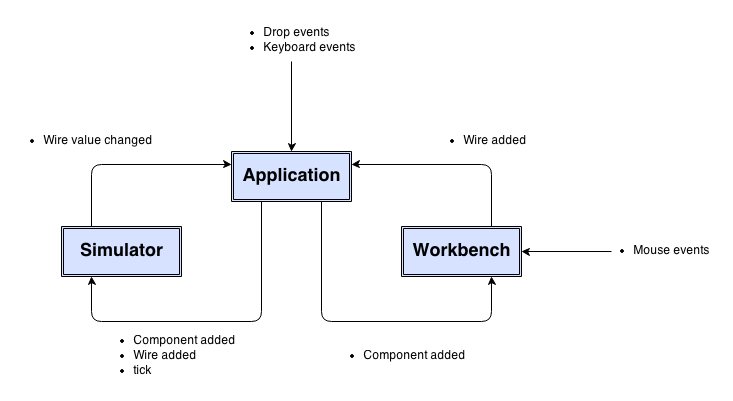
\includegraphics[width=\textwidth]{application.png}
    \caption{Information flow in GatePlay}
    \label{fig:application}
\end{figure}


\subsection{application.js}

\clearpage
\chapter{Testing}
Testing is extremely important in the development of non-trivial programs. Tests give some assurance to the correctness of the code, and highlight \textit{regressions} (where code that used to work is broken by a recent change) quickly.

\section{Unit Testing}
Unit testing is used to test the correctness of small modules of code, such as functions. The simulator has a suite of unit tests. One example is a test over the $AND$ evaluation function shown in figure~\ref{fig:andtest}. All \textit{evaluate} functions had to be changed when $Blinker$s were implemented, and this test flagged a regression when the first implementation had a bug.

\begin{figure}
\begin{lstlisting}[language=JavaScript]
var T = TruthValue.TRUE;
var F = TruthValue.FALSE;
var U = TruthValue.UNKNOWN;

function ANDTest() {
	var and = Functions.get("and");	
	
	// Test 2-input truth table
	equal(and.evaluate([T,T]), T);
	equal(and.evaluate([T,F]), F);
	equal(and.evaluate([T,U]), U);
	equal(and.evaluate([F,T]), F);
	equal(and.evaluate([F,F]), F);
	equal(and.evaluate([F,U]), F);
	equal(and.evaluate([U,T]), U);
	equal(and.evaluate([U,F]), F);
	equal(and.evaluate([U,U]), U);
}
\end{lstlisting}
\caption{Testing $AND$'s truth table}
\label{fig:andtest}
\end{figure}

Unit tests are also very useful for catching simple bugs in frequently edited code. For example, the \textit{tick} function in the circuit simulator is responsible for handling all events which occur at the current time, and them increments the current time. Since the \textit{tick} function is so frequently modified, it is easy to introduce simple bugs. The test shown in figure~ simply checks that the system clock is incremented after \textit{tick} is called.

I used a common JavaScript unit testing framework QUnit\footnote{http://qunit.com} to reduce the boilerplate in writing unit tests.

\section{End-to-end Testing}
Unit testing is a bottom-up approach which checks that the smallest modules work as expected in isolation. End-to-end testing is a top-down approach which
\clearpage
\chapter{Conclusions}

\clearpage
\begin{thebibliography}{9}

\bibitem{logicly} http://logic.ly.

\end{thebibliography}

\end{document}